\section{UC6: Search, Filter, and Pagination}

\begin{figure}[H]
\centering
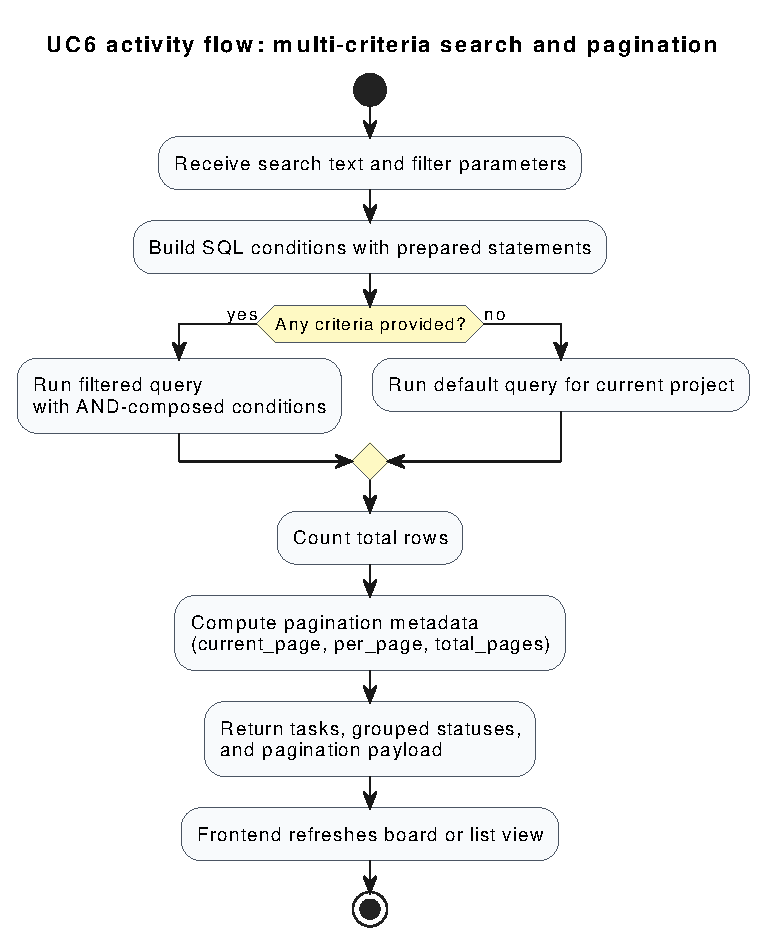
\includegraphics[width=\textwidth,height=0.82\textheight,keepaspectratio]{diagrams/generated/uc6-search-filter-flow.pdf}
\caption{UC6 activity flow: multi-criteria search and pagination}
\label{fig:uc6-search-filter-flow}
\end{figure}


\subsection{Search and Filter Model}

Search and filtering are handled by \code{includes/task-functions.php} (\code{searchProjectTasks}, \code{searchGetFilterOptions}) and routed through \code{api/tasks.php}.
Supported criteria:
\begin{itemize}
    \item Text search in task title and description.
    \item Single-value filters for status, priority, and assignee.
    \item Due date range filters.
    \item Extra presets such as overdue and due-this-week conditions.
\end{itemize}

\subsection{Pagination Contract}

The API returns paginated metadata:
\begin{itemize}
    \item \code{current\_page}, \code{per\_page}, \code{total\_items}, \code{total\_pages}.
    \item \code{has\_prev} and \code{has\_next} flags for UI navigation.
\end{itemize}

This prevents large response payloads and keeps board rendering responsive when task volume increases.

\screenshotplaceholder{Search and filter modal with multi-criteria options}{search-filter-modal.png}
